%# -*- coding: utf-8-unix -*-

\chapter{结合共享账户的机票推荐算法}
\label{chap:share}

本章我们研究机票推荐中的共享账户问题,该问题主要针对一个用户ID包括多个乘客的情况。我们将提出一种算法,可以预测出用户下本次购票的乘客的概率分布,从而学习更具针对性的偏好模型,提升推荐准确率。

\section{机票推荐中的共享账户}

推荐算法总体分为两类,一类是根据用户和物品之间的关系,提出衡量用户相似度以及物品相似度的算法,为用户根据物品或用户之间的相似度提供推荐结果;另一类是基于内容的推荐,物品可以表示为特征的集合(包括显性特征和隐性特征),从用户的物品列表中学习用户对每个特征的偏好。为用户推荐最符合其特征偏好的物品。

以这两类算法为代表的传统推荐系统通常以用户在网站的注册ID(账户)来识别用户,它们一般假定一个用户背后只有一个使用者,即每个用户仅包含一个固定的偏好模型。然而在很多领域,都会发生现实中几个人共同使用一个账户的情景。例如,在购物网站,可能一个家庭共用一个账户,每位家庭成员都可以使用这个账户进行购物;在一般的线旅行票务服务网站,例如机票、酒店、旅游等业务领域,一个账户中也可能会有几个成员,他们可能会为家人、旅伴购票。


第一种情形中,虽然会有几位家庭成员共同使用账户购物,但是服务商无法获取购物者的真实身份信息。而对于第二种情形,如图\ref{fig:fill_id}所示,乘客在订票后会被要求填写身份信息,因此,网站可以获取其真实身份。在机票数据集中,订单包含了每一位乘客的身份信息,包括姓名、性别、年龄、证件号码等。在我们进行数据分析与实验过程中,统一使用加密后的证件号码来代指乘客,既确保了乘客之间无冲突,又保护了乘客隐私。

\begin{figure}
 \centering
 \includegraphics[width=0.5\linewidth]{05/1_fill_id.png}
 \bicaption[fig:fill_id]{填写乘客信息}{用户在票务网站填写身份信息}{Fig}{Users Fill in Their Identification on Website}
\end{figure}

通常来说,同一个用户下乘客可能具有较为相似的偏好,但他们之间的差异也不能忽视。如果我们能够利用购票时获取的乘客身份信息为该乘客进行机票推荐,就可以为每位乘客建立特征分布模型,更具针对性的细粒度乘客模型对进一步提升个性化机票推荐准确率可以起到作用。然而,按照业务流程,只有当用户选定机票后才会填写身份信息。在我们进行机票推荐时还无法获取乘客信息。我们需要预测乘客的概率分布。

我们的问题是在共享账户的乘客选购机票时,根据乘客历史行为模式以及当前会话的上下文预测出本次购票的目标乘客。在电子购物网站等无法获得成员真实身份的场景中,为了解决共享账户问题,通常需要设置几个虚拟成员,其中每个成员代表一种偏好模型。虚拟成员的数量可以是固定值,也可以是通过模型计算出的最优值。然而,这类算法通常只分析用户和物品之间的关系,无法利用当前会话中的上下文信息;并且对虚拟成员预测的分布准确率也无法验证。在机票推荐场景中,对乘客的预测准确率是可以进行验证的。

在机票的乘客预测模型中,我们使用了作者主题模型(ATM)来分析乘客的行为模型。主题模型是一种生成模型,其主要观点是一篇文档可以抽取出混合的多个主题。作者主题模型在原主题的基础上又添加了作者的关系。每个账户独立进行模型训练,可以将每个账户看作一个语料库。账户中出现过的所有乘客看作每位作者,每条机票订单看作一篇文档, 机票中的每个特征以及上下文信息看作预定义的词库。如果出现一张机票有多个乘客的情况,我们将他们视为共同作者。

\section{乘客预测模型}
事实上,主题模型在推荐系统中的应用很广泛。例如,在pLSA模型中,每个物品可以视作一个词汇,主题服从对物品的多项式分布,每个主题代表了一种隐性特征。每用户的偏好模型都服从对主题的多项式分布。用户的每次购买行为都可以被看作从该用户中抽样一个主题$Z$,再从该主题中抽取一个词汇的过程。由于机票具有动态属性,很难将不同价格的机票定义为同一个物品;并且每类机票的数量受限于飞机的型号,因此上述pLSA模型很难用到机票推荐领域中。

\subsection{模型描述及表示}

在作者主题模型中,我们用机票在每个特征离散化后的取值来预定义一个词库。这个词库包含了机票在任一特征中所有可能出现的值,使用从0开始的索引来代指每一个词汇。至此,每一张机票都可以表示为词汇的集合,我们将每条订单视作一篇文档,显然,所有文档的词汇数量都是相同的。每个主题都由词汇的多项式分布表示;类似地,每个乘客由主题的多项式分布表示。因此
ATM模型可以对文档(订单)进行降维。通过模型训练,可以计算出乘客与主题之间的分布参数以及主题与词汇之间的分布参数。表\ref{tab:notation}描述了我们本章使用的符号表。

\begin{table}[!hpb]
\centering
  \bicaption[tab:notation]{符号表}{乘客预测模型符号表}{Table}{Notation for ATM}
\begin{tabular}{|c|c|} \hline
$M$ & 数据集账户数量\\ \hline
$V$ & 词汇表中单词的数量\\ \hline
$O$ & 一个账户中所有订单\\ \hline
$P$ & 一个账户中所有乘客\\ \hline
$P_i$ & 订单$O_i$对应的乘客集合 \\ \hline
$F$ & 机票特征集合\\ \hline
$K$ & 主题数量\\ \hline
\end{tabular}
\end{table}

对于一个账户$M$,我们获取其中包含的乘客集合$P$。我们使用矩阵$\Theta$来表示每位乘客的主题分布,这个参数矩阵的维度是$|P| \times K$,$K$代表模型主题的数量。$\Theta$以狄利克雷分布作为先验,该先验的超参数是$\alpha$。矩阵$\Phi$可以表示每个主题在词汇上的分布,该矩阵的维度是$V \times K$。$\Phi$同样以超参数为超参数是$\beta$的狄利克雷分布作为先验。通常情况下,超参数不是通过训练得到的,而是根据多次数据实验的经验总结来赋值。本章中,我们将$\alpha$赋值为$50/K$,将$\beta$赋值为0.01。

式\ref{eq:dir}描述了狄利克雷分布。其中,带$\Gamma$函数的那一项是常系数。可以发现,狄利克雷分布与多项式分布具有相同的形式。这两个分布是共轭分布。

\begin{eqnarray}
\label{eq:dir}
	Dir(\mathbf{p}|\alpha) & = & \frac{1}{B(\alpha)}\prod_{i=1}^n p_i^{\alpha_i-1} \nonumber \\
	& = & \frac{\Gamma(\sum_{i=1}^n \alpha_i)}{\prod_{i=1}^n \Gamma(\alpha_i)}\prod_{i=1}^n p_i^{\alpha_i-1}
\end{eqnarray}

在训练数据中,一条机票订单的乘客集合是明确的,每张机票的特征内容,即该篇文档的所有词汇也是明确的;为了训练两个矩阵参数,我们需要为文档中的每个词汇赋予乘客与主题。这两个变量属于隐性变量。首先我们从这条订单的乘客列表中按均匀分布抽取出一位乘客;然后根据乘客-主题参数矩阵抽取出一个主题$Z$,再根据主题-词汇参数矩阵抽取一个单词$w$,我们使用下列流程对生成模型进行数学描述:

\begin{enumerate}
\item 对每个账户中的所有乘客$p$,以狄利克雷先验初始化 $\Theta_p \sim Dir(\alpha)$
\item 对每个主题$t$,以狄利克雷先验初始化 $\Phi_t \sim Dirichlet(\beta)$
\item 对账户下的每条订单$o$
       \begin{enumerate}[fullwidth,itemindent=1em,label=(\alph*)]
       \item $P$ 表示这条订单的乘客集合
       \item 对于订单中的每一个词汇
              \begin{enumerate}[fullwidth,itemindent=2em,label=(\roman*)]
              \item 按均匀分布从$P$中抽取一位乘客 $X_{oi} \sim Uniform(P)$
              \item 从乘客-主题矩阵中抽取一个主题 $Z_{oi} \sim Discrete(\theta_{X_{oi}})$
              \item 从主题-词汇矩阵中抽取一个单词 $w_{oi} \sim Discrete(\phi_{Z_{oi}})$
              \end{enumerate}
       \end{enumerate}
\end{enumerate}

图\ref{fig:pro_graph}展示了作者主题模型的概率图。带阴影的变量是已知变量;其余是未知变量。每个方框代表一个过程,其右下角的数字是这个过程的循环次数。箭头连接线代表了变量间的条件依赖关系。这个图直观、清晰地表现了生成一篇文档的过程。

\begin{figure}
 \centering
 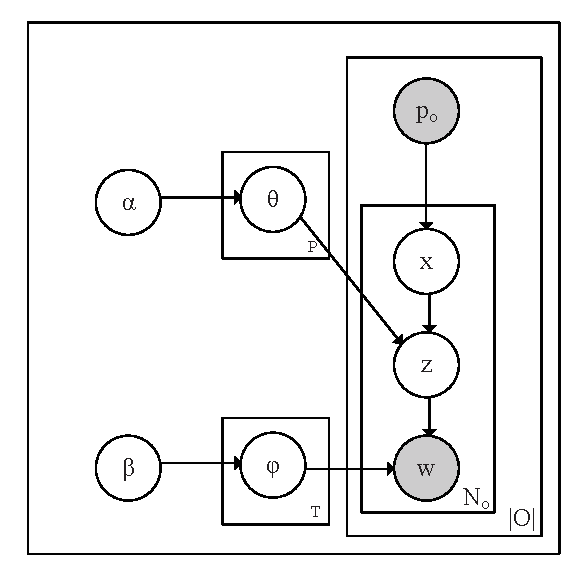
\includegraphics[width=0.45\linewidth]{05/2_graph.eps}
 \bicaption[fig:pro_graph]{模型概率图}{作者主题模型的概率图}{Fig}{Probability Graph for the Author-topic Model}
\end{figure}

\subsection{模型参数推导}
在上节的模型描述中,我们介绍了作者主题模型的两个参数矩阵,分别是包含$P$位乘客的乘客-主题分布参数以及包含$K$个主题的主题-词汇分布。有一些算法可以用来推导这些参数,如EM算法、Gibbs采样等。传统的EM算法可能会陷入局部最优问题,并且这种算法的计算复杂性较高。本章,我们使用Gibbs采样的算法,这种算法不直接进行参数推导,而通过计算抽取的乘客和主题的后验分布,对参数进行更新。因此计算过程较为简单。


\begin{eqnarray}
\label{eq:all_pro}
P(\mathbf{w}_o | \Theta,\Phi,P) & = & \prod_{i=1}^{N_o}P(w_{oi}|\Theta,\Phi,\mathbf{p}_o) 
\nonumber \\
 & = & \prod_{i=1}^{N_o}\sum_{p=1}^{|P|}\sum_{t=1}^{K}P(w_{oi}|z_{oi}=t,\Phi)
P(z_{oi}=t|x_{oi}=p,\Theta)P(x_{oi}=p|\mathbf{p}_o) \nonumber \\
 & = & \prod_{i=1}^{N_o}\frac{1}{|P|}\sum_{p \in p_o}\sum_{t=1}^{K}\phi_{w_{oi}t}\theta_{tp}
\end{eqnarray}


式\ref{eq:all_pro}描述了在参数矩阵$\Theta$,$\Phi$和乘客集合$P$的条件下,生成一条机票订单的概率函数。在这个生成模型中,$P(w_{oi}|z_{oi}=t,\Phi)$是在选定主题的条件下,根据主题-词汇分布矩阵抽取单词的概率。
$P(z_{oi}=t|x_{oi}=p,\Theta)$是在选定乘客的条件下,根据乘客-主题分布矩阵抽取主题的概率。$P(x_{oi}=p|\mathbf{p}_o)$是乘客集合中以服从均匀分布抽取乘客的概率。这个等式可以看作生成一条订单的似然函数。如果将参数$\Theta$,$\Phi$视为随机变量,我们训练模型的目标就是训练变量,使概率函数具有最大后验分布(MAP, Maximum A Posteriori)。 

在Gibbs采样的过程中,为了从联合分布$P(\mathbf{z},\mathbf{x}|\alpha,\beta)$中取样,我们需要为每一个单词$w_{di}$赋值一个主题$z_{di}$以及乘客$x_{di}$。在训练过程中,一个账户下的所有单词都会被取样一次。当所有单词都训练过,称为一个训练批次。通常,我们需要将模型训练数个批次。$p(\Theta,\Phi|\mathbf{z},\mathbf{x},\alpha,\beta)$可以根据狄利克雷和多项式分布四共轭分布的性质来计算。为每个单词抽取的乘客、主题可以使用下式进行计算:

\begin{eqnarray}
\label{eq:p_xz}
P(x_{oi}=p,z_{oi}=t|w_{oi}=w,\mathbf{z}_{-oi},\mathbf{x}_{-oi},\mathbf{w}_{-oi},\alpha,\beta,p_o) \nonumber\\
\propto \frac{C_{tp}^{TP}+\alpha}{\sum{t'}C_{t'p}^{TP}+T\alpha}\frac{C_{wt}^{WT}+\beta}{\sum_{w'}C_{w't}^{WT}+W\beta}
\end{eqnarray}

式\ref{eq:p_xz}代表为订单$o$的第i个单词赋予乘客p和主题t的概率。$C^{WT}$ 是单词-主题分布矩阵,其每行对应一个单词,每列对应一个主题,每个值代表当前单词被赋予当前主题的次数。$C_{wt}$是除了当前单词之外,单词$w$被赋予主题$t$的次数。$C^{TP}$是主题-乘客分布矩阵,其每行对应一个主题,每列对应一个乘客,矩阵中每个值代表对与该乘客在当前主题包含的单词个数。$C_{tp}$代表乘客$p$在主题$t$包含的词汇个数,同样排除了当前单词。我们可以根据抽样的过程对主题-词汇分布参数以及乘客-主题分布参数进行更新:

\begin{equation}
\label{eq:es_the}
\theta_{tp} = \frac{C_{tp}^{TP}+\alpha}{\sum{t'}C_{t'p}^{TP}+T\alpha}
\end{equation}

\begin{equation}
\label{eq:es_phi}
\phi_{wt} = \frac{C_{wt}^{WT}+\beta}{\sum_{w'}C_{w't}^{WT}+W\beta}
\end{equation}

式\ref{eq:es_the}和式\ref{eq:es_phi}分别两个参数的更新公式。$\theta_{tp}$是主题t在乘客p上的概率分布;$\phi_{wt}$是单词w在主题t上的概率分布。因此,在参数推导的过程中,我们还需存储两个矩阵,分别是上文提到的$C^{TP}$和$C^{WT}$。

%1.参数更新
%2.总体描述 && 算法
%3.乘客预测

\section{结合乘客预测的机票个性化推荐}
总体流程图
%???权重训练 &&算法
评价指标
预测结果
推荐结果



\section{实验结果分析}

\section{本章小结}